\documentclass[12pt,letterpaper]{article}

% ---------- Packages ----------
\usepackage[letterpaper,margin=1in]{geometry}
\usepackage[T1]{fontenc}
\usepackage[utf8]{inputenc}
\usepackage{newtxtext,newtxmath} % Times-like font
\usepackage{microtype}
\usepackage{graphicx}
\usepackage{booktabs}
\usepackage{array}
\usepackage{tabularx}
\usepackage{enumitem}
\usepackage{titlesec}
\usepackage{xcolor}
\usepackage{hyperref}
\usepackage{fancyhdr}

% ---------- Colors (from Aspose export) ----------
\definecolor{brand}{rgb}{0.478431,0,0.235294}   % color_147093
\definecolor{accent}{rgb}{0.67451,0.078431,0.333333} % color_195788
\definecolor{textgray}{rgb}{0.2,0.2,0.2}        % color_80434
\definecolor{rulegray}{rgb}{0.866667,0.866667,0.866667} % color_249244

% ---------- Document styling ----------
\hypersetup{colorlinks=true,linkcolor=brand,urlcolor=accent,citecolor=brand}
\pagestyle{fancy}
\fancyhf{}
\lhead{}
\rhead{}
\lfoot{SE/CS 3RA3 — Fall}
\rfoot{\thepage}
\renewcommand{\headrulewidth}{0pt}
\renewcommand{\footrulewidth}{0.4pt}

\titleformat{\section}{\Large\bfseries\color{brand}}{\thesection}{0.75em}{}
\titleformat{\subsection}{\large\bfseries\color{brand}}{\thesubsection}{0.75em}{}
\titleformat{\subsubsection}{\normalsize\bfseries\color{brand}}{\thesubsubsection}{0.75em}{}

\setlist[itemize]{topsep=4pt,itemsep=2pt,parsep=0pt}
\setlist[enumerate]{topsep=4pt,itemsep=2pt,parsep=0pt}

% ---------- Title page ----------
\makeatletter
\def\@maketitle{%
  \begin{center}
    \vspace*{1.5cm}
    {\Huge\bfseries\color{brand} Our Awesome Project\par}
    \vspace{0.35cm}
    {\Large\itshape\color{accent} Requirements Standard Plan\par}
    \vspace{0.9cm}
    {\large Saad Salman, Author 2, Author 3\par}
    \vspace{0.25cm}
    {\normalsize Version 1, 2025-09-22\par}
    \vspace{1.5cm}
  \end{center}
}
\makeatother
\title{}
\author{}
\date{}

\begin{document}
\maketitle
\thispagestyle{empty}
\clearpage

\tableofcontents
\clearpage

% ---------- Academic Integrity Disclaimer ----------
\section*{Academic Integrity Disclaimer}
\addcontentsline{toc}{section}{Academic Integrity Disclaimer}
We would like to acknowledge that as dedicated students of McMaster University, we have thoroughly read and comprehended the Academic Integrity Policy published by the university. We are committed to upholding the principles of academic honesty and integrity in all aspects of our educational journey. We understand the importance of acknowledging the work and ideas of others, and we pledge to ensure that all our academic endeavors are conducted with the utmost originality and compliance with the university’s policy.

We affirm that the content presented in this document is entirely our own, and any external sources used have been appropriately cited and referenced.

\medskip
\noindent\textbf{Saad Salman} \\
As I submit my work, I, Saad Salman, take full responsibility for the integrity of my work and promise to avoid any form of plagiarism, cheating, or dishonest behavior. This acknowledgment serves as a testament to my dedication to academic excellence and the fostering of a trustworthy academic community at McMaster University.

\medskip
\noindent\textbf{Author 2} \\
As I submit my work, I, Author 2, take full responsibility for the integrity of my work and promise to avoid any form of plagiarism, cheating, or dishonest behavior. This acknowledgment serves as a testament to my dedication to academic excellence and the fostering of a trustworthy academic community at McMaster University.

\medskip
\noindent\textbf{Author 3} \\
As I submit my work, I, Author 3, take full responsibility for the integrity of my work and promise to avoid any form of plagiarism, cheating, or dishonest behavior. This acknowledgment serves as a testament to my dedication to academic excellence and the fostering of a trustworthy academic community at McMaster University.

\medskip
\noindent\textit{Policy:} \url{https://secretariat.mcmaster.ca/app/uploads/Academic-Integrity-Policy-1-1.pdf}

\clearpage

% ---------- Control Information ----------
\section{Control Information}
\begin{table}[h!]\centering
\caption*{Versioning and Delivery}
\renewcommand{\arraystretch}{1.2}
\begin{tabularx}{\textwidth}{@{}l l l l l l@{}}
\toprule
\textbf{Version} & \textbf{Delivery Deadline} & \textbf{Delivered} & \textbf{Feedback Received} & \textbf{Integrated} & \textbf{Notes} \\
\midrule
V1 & & & & & \\
V2 & & & & & \\
V3 & & & & & \\
\bottomrule
\end{tabularx}
\end{table}

\medskip
\noindent\textbf{Saad Salman} \\
Here is a quick biography of Saad Salman. You can contact them at \href{mailto:salmam12@mcmaster.ca}{salmam12@mcmaster.ca}.

\medskip
\noindent\textbf{Author 2} \\
Here is a quick biography of Author 2. You can contact them at \href{mailto:a2@mcmaster.ca}{a2@mcmaster.ca}.

\medskip
\noindent\textbf{Author 3} \\
Here is a quick biography of Author 3. You can contact them at \href{mailto:a3@mcmaster.ca}{a3@mcmaster.ca}.

\clearpage

% ---------- (G) Goals ----------
\section{(G) Goals}
\subsection*{Reading Guide}
Goals are ``needs of the target organization, which the system will address''. While the development team is the principal user of the other books, the Goals book addresses a wider audience: essentially, all stakeholders \cite{meyer2022}. It must contain enough information to provide---if read just by itself---a general sketch of the entire project. To this effect, chapter G.3 presents a short overview of the system and G.1 will typically include some key properties of the environment. As it addresses a wide readership, it should be clear and minimize the use of specialized technical terms. Together, G.1, G.2 and G.3 describe the rationale for the project. It is important to state these justifications explicitly. Typically, they are well understood at the start of the project, but management and priorities can change \cite{meyer2022}.

\subsection*{Control Information}
\begin{table}[h!]\centering
\caption*{Table 1. Our Awesome Project --- Versioning Information --- Goal Book}
\renewcommand{\arraystretch}{1.1}
\begin{tabularx}{\textwidth}{@{}l l l l l l@{}}
\toprule
\textbf{Section} & \textbf{Version} & \textbf{Lead} & \textbf{Delivered on} & \textbf{Reviewer} & \textbf{Approved on} \\
\midrule
G.1 & M1 & SS & Sept-21-2025 & SP & Sept-22-2025 \\
G.2 & M1 & SS & Sept-21-2025 & SP & Sept-22-2025 \\
G.3 & & & & & \\
G.4 & & & & & \\
G.5 & & & & & \\
G.6 & & & & & \\
G.7 & & & & & \\
\bottomrule
\end{tabularx}
\end{table}

\subsection{(G.1) Context and Overall Objectives}
Commuting to McMaster University presents significant financial and environmental challenges. Students, staff, and faculty spend between 150 and 250 dollars monthly on fuel, parking, or transit, which places an economic burden on them. At the same time, single-occupancy vehicles contribute to 36 percent of greenhouse gas emissions for Canadian universities, harming both local air quality and broader sustainability goals. Existing ridesharing solutions such as Facebook Marketplace, Kijiji, or Poparide do not provide sufficient verification or security, leaving users at risk of riding with unaffiliated strangers. The objective of Hitchly is to provide a safe, affordable, and reliable ridesharing platform tailored for the McMaster community. By verifying users through McMaster email accounts, Hitchly ensures trust, reduces costs, supports sustainability, and helps the university meet its long-term community and environmental goals. 

\subsection{(G.2) Current Situation}
Currently, McMaster commuters lack a centralized, trusted platform to connect drivers and riders within the university community. Those who rely on driving face steep monthly costs for gas and parking, while those taking transit encounter expensive or unreliable services. Informal ridesharing options exist, but they provide limited safety features and lack institutional alignment, making them unsuitable for building long-term trust. Students and staff often feel that available solutions are unsafe, inefficient, or financially burdensome. Hitchly seeks to fill this gap by providing a McMaster-specific application that facilitates secure ridesharing, reduces commuting costs, and lowers emissions. 

\subsection{(G.3) Expected Benefits}
The pilot delivers clear, stakeholder-visible outcomes. Riders should see more affordable commutes (targeting approximately 20\% savings) while drivers receive meaningful cost offsets (around 40\%). We aim for reliable availability ($\geq$70\% ride-fill and $\geq$95\% on-time) so trips feel predictable from day one, with most new users completing a first ride within a week. The pilot targets a reduction in single-occupancy trips on campus and nearby (aiming for at least 10\%), easing parking pressure and congestion and reducing emissions. The service will be inclusive by default (targeting about 90\% match on stated accessibility preferences) and trusted through university-verified identities with a goal of very low incident rates. The university benefits from higher student satisfaction and sense of belonging, improved commuter equity, and better alignment with sustainability reporting---while maintaining privacy safeguards (goal: zero critical incidents). Broader community outcomes include cleaner air, calmer peak traffic, and greater participation in transit and shared mobility.

\begin{figure}[htbp]
  \centering
  % path is relative to the .tex file; create docs/SRS/images/ and put your file there
  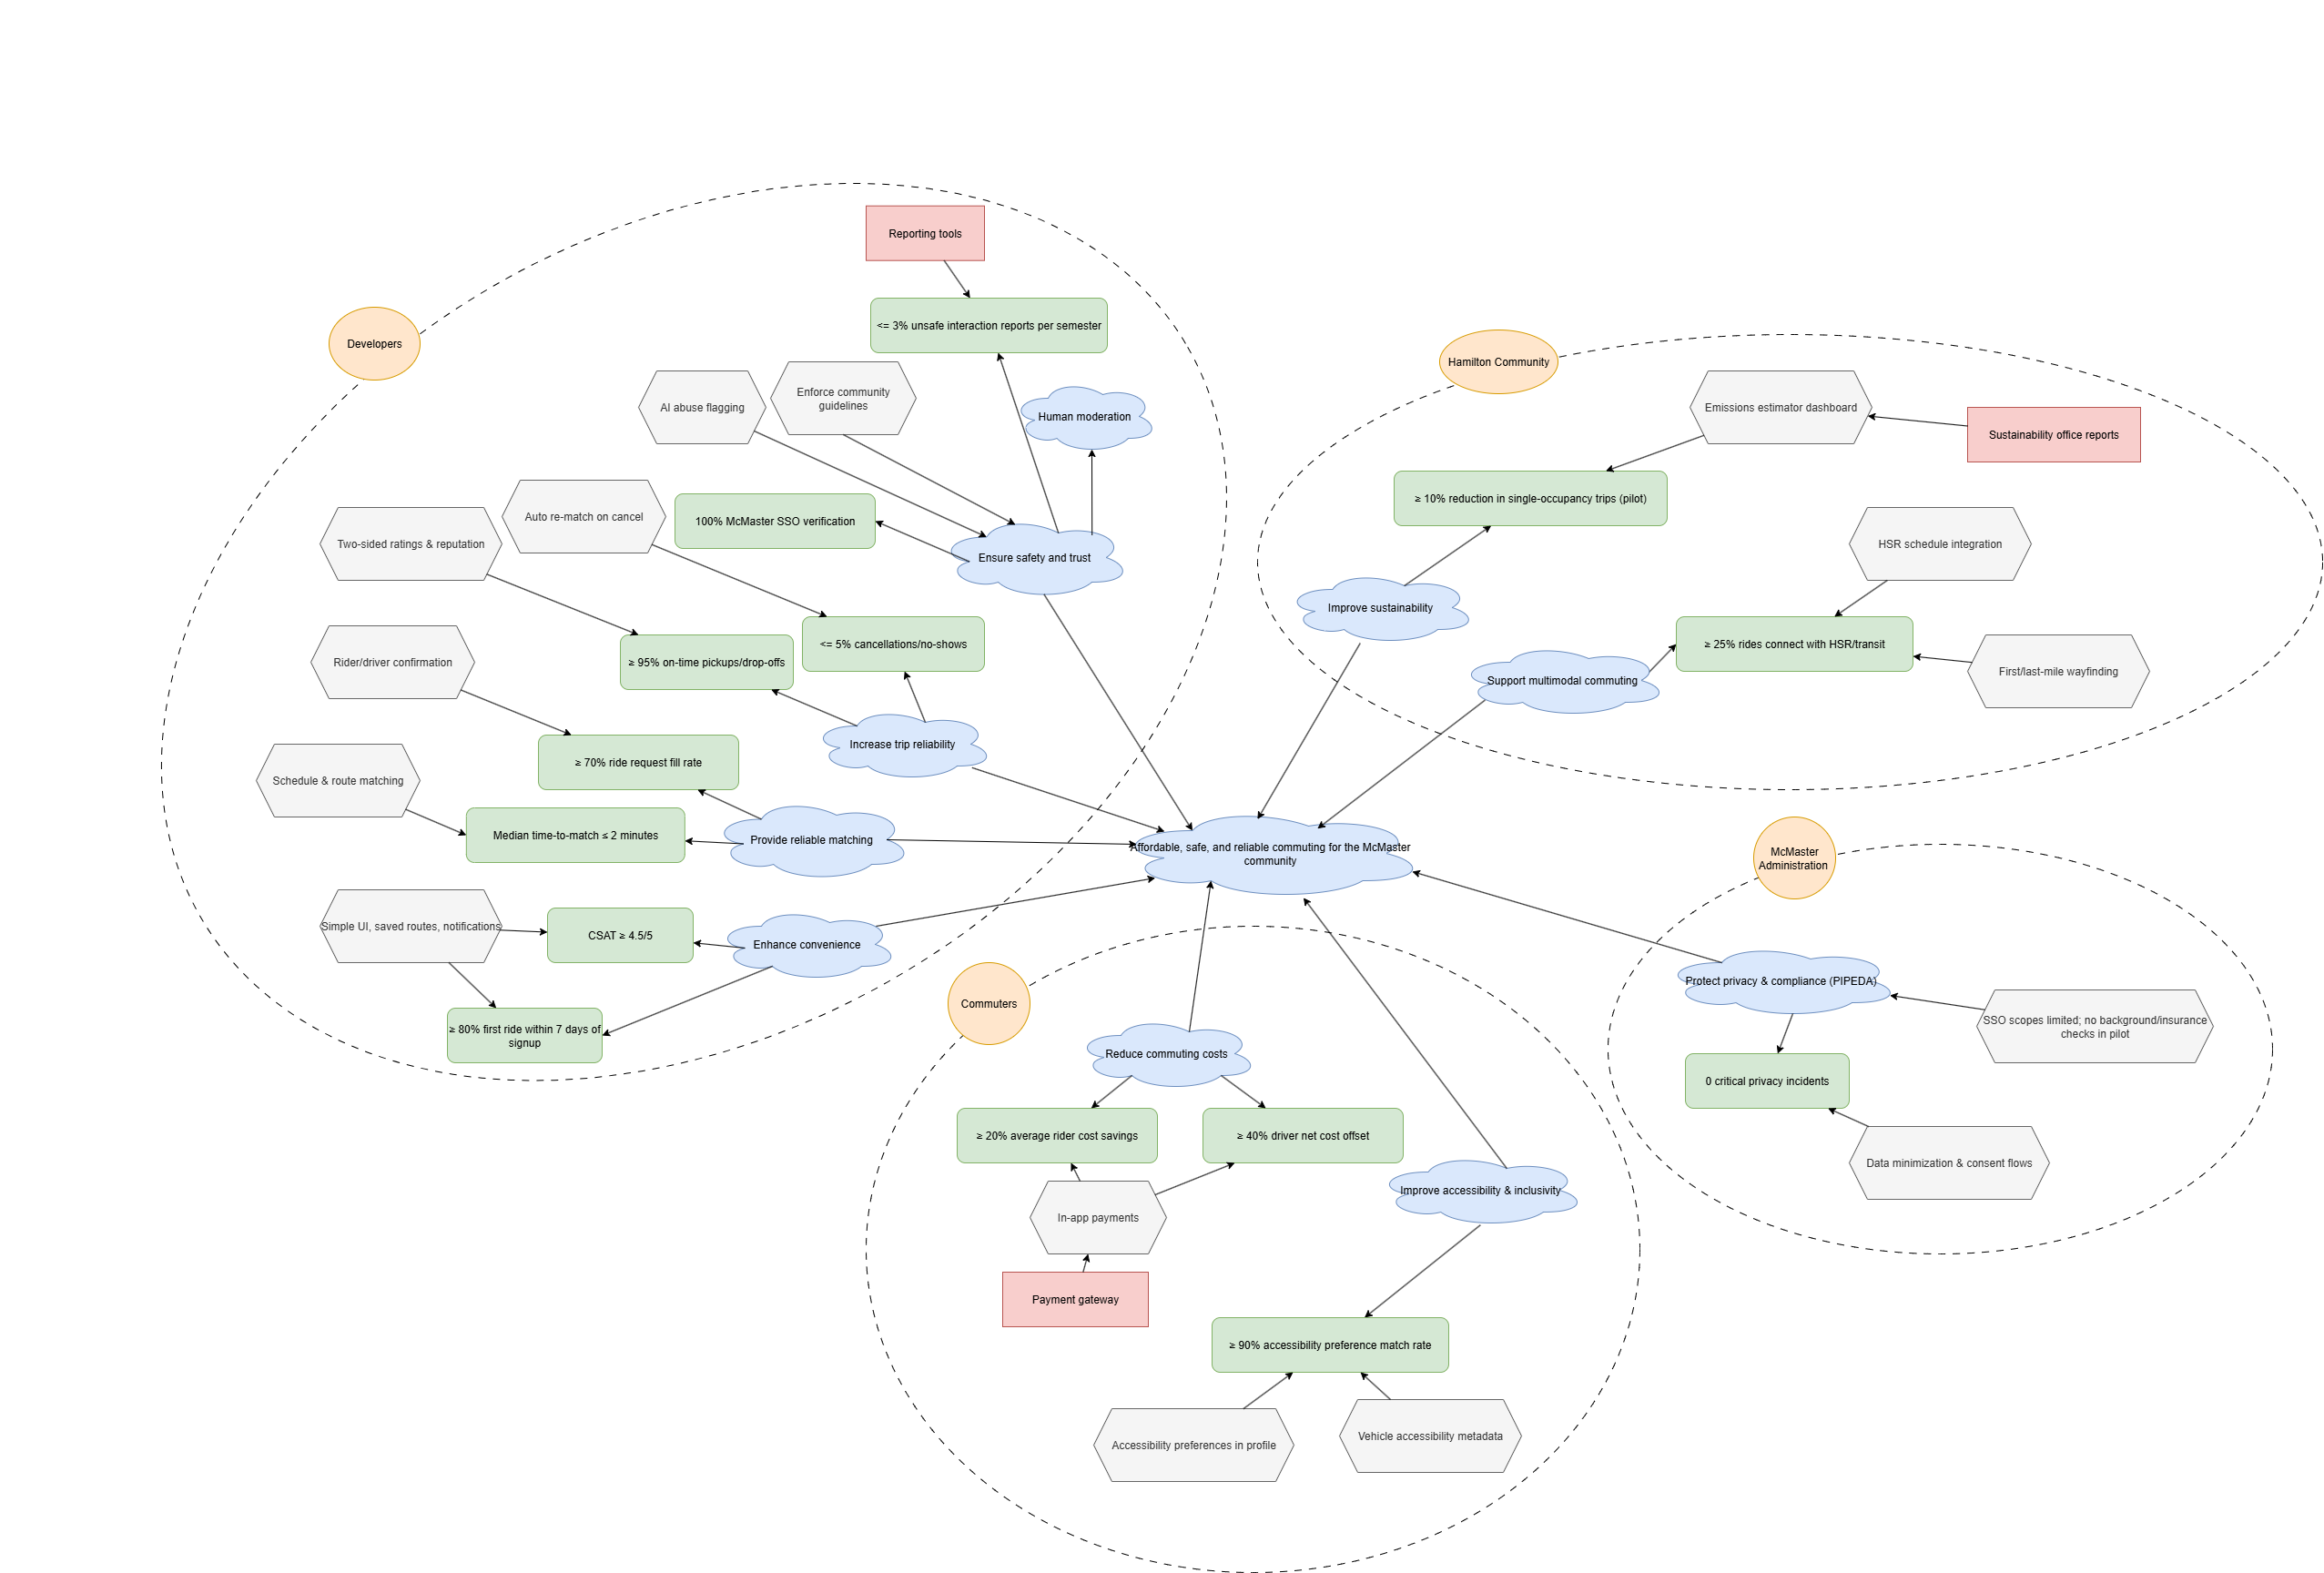
\includegraphics[width=0.75\textwidth]{goal_model.png}
  \caption{Hitchly Goal Modelling Diagram.}
  \label{fig:ride-matching}
\end{figure}

\textit{Nothing available at this point.}

\subsection{(G.4) Functionality Overview}
Overview of the functions (behavior) of the system. Principal properties only (details are in the System book). A capsule version of book S that enables readers to get a quick grasp of what the system will do \cite{meyer2022}.

\textit{Nothing available at this point.}

\subsection{(G.5) High-level Usage Scenarios}

\subsubsection*{Use Case 1: Driver Offers Ride}
\begin{enumerate}
    \item A driver registers with their McMaster email and drivers license.
    \item They input their schedule and vehicle details.
    \item Hitchly suggests potential riders with overlapping times.
    \item The driver confirms the riders they want to take.
    \item The system calculates cost-sharing estimates.
    \item After the trip, the driver receives ratings and reviews.
\end{enumerate}

\subsubsection*{Use Case 2: Rider Finds Ride}
\begin{enumerate}
    \item A rider signs up with a McMaster email.
    \item They enter their daily commute times and location.
    \item Hitchly presents a list of verified drivers with compatible schedules.
    \item The rider selects a driver and confirms.
    \item The system provides trip details, including cost share.
    \item After the ride, the rider leaves a review.
\end{enumerate}

\subsubsection*{Use Case 3: Report Safety Issue}
\begin{enumerate}
    \item A rider feels unsafe during a trip.
    \item They submit a report through the in-app reporting tool.
    \item Hitchly forwards the report to moderators.
    \item The moderators review and investigate the case.
    \item The driver’s or rider’s account is flagged if necessary.
    \item The system tracks the resolution and stores it for accountability.
\end{enumerate}

\subsubsection*{Use Case 4: Sustainability Tracking}
\begin{enumerate}
    \item Hitchly logs each completed trip.
    \item The system calculates estimated emissions avoided.
    \item Data is aggregated in dashboards.
    \item McMaster administration reviews statistics to measure impact.
    \item The results inform sustainability planning.
    \item Reports can be shared with the broader community.
\end{enumerate}

\begin{figure}[htbp]
  \centering
  % path is relative to the .tex file; create docs/SRS/images/ and put your file there
  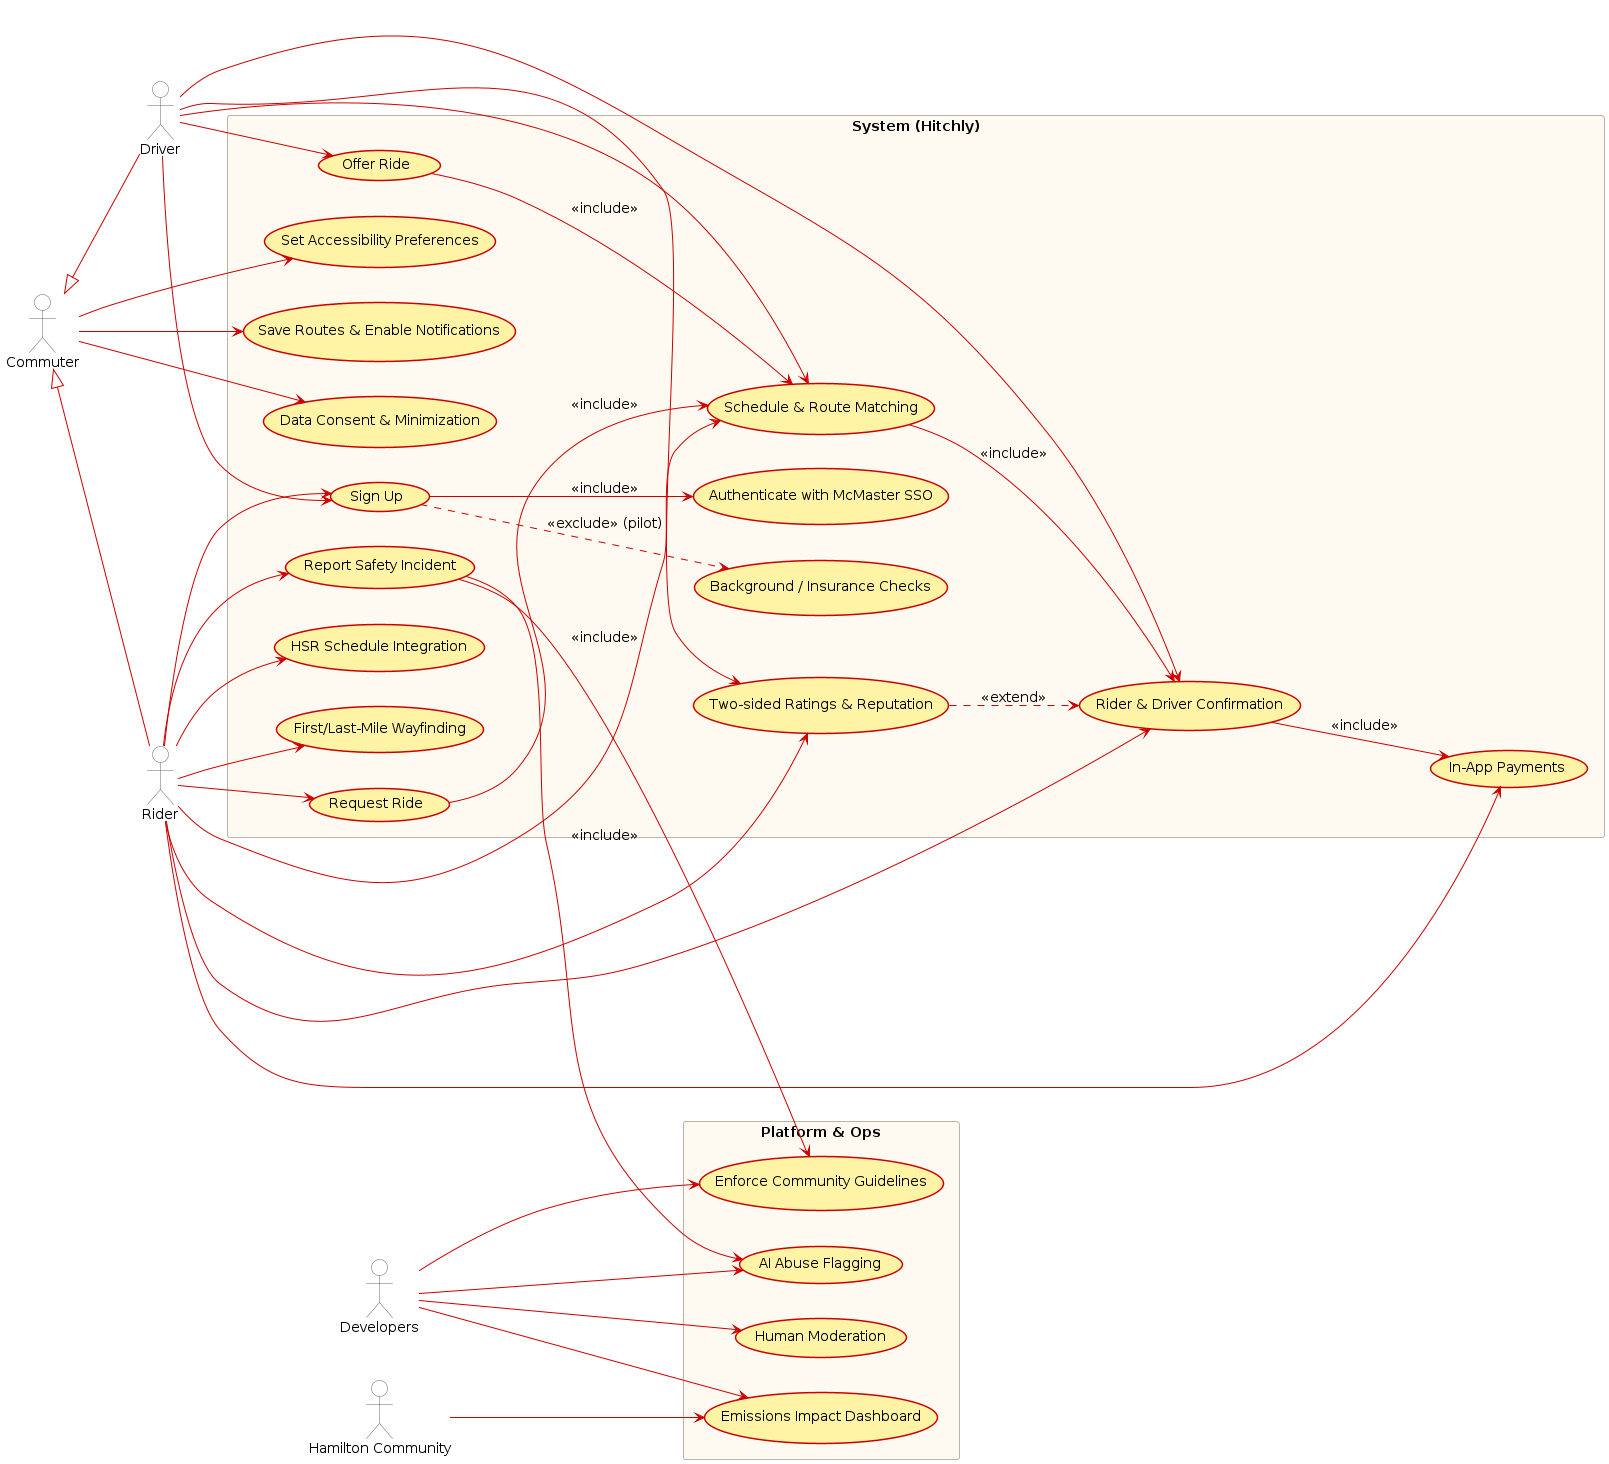
\includegraphics[width=0.75\textwidth]{use-case.png}
  \caption{Hitchly Use Case Diagram.}
  \label{fig:ride-matching}
\end{figure}

\subsection{(G.6) Limitations and Exclusions}
\begin{itemize}
  \item McMaster-Only Access: Hitchly will only be available to McMaster students, staff, and faculty during the pilot phase. Users must verify their identity through a McMaster email. This restriction ensures trust and control but limits the platform’s reach to a single institution. 

  \item Background and Insurance Checks: For the pilot phase, Hitchly will not perform in-depth background checks or validate driver insurance. Verification is limited to McMaster email zn d driver license authentication. This keeps onboarding simple but places responsibility on users to ensure their own compliance with driving regulations.

  \item Limited Route Flexibility: Hitchly will not provide dynamic routing or live GPS tracking during the pilot. Riders and drivers must coordinate based on general pickup and drop-off locations. This simplifies the system but may limit convenience compared to fully featured ridesharing platforms. 
\end{itemize}


\subsection{(G.7) Stakeholders and Requirements Sources}

\subsubsection*{Direct Stakeholders}

\paragraph{Students}
They are frequent commuters with tight budgets who will use Hitchly to save money and connect with peers. 
Relevant because they face high monthly commuting costs.\\
\textbf{Persona:} ``Sarah, a second-year student living off-campus, spends over \$200 monthly on commuting. She uses Hitchly to reduce expenses and meet fellow students traveling the same route.''

\paragraph{Staff}
Staff members travel daily to campus and benefit from both cost savings and reduced parking stress. 
Relevant because they often drive alone and bear significant expenses.\\
\textbf{Persona:} ``James, a staff member living in Burlington, drives to McMaster five days a week. Hitchly allows him to share costs and avoid the hassle of finding parking.''

\paragraph{Faculty}
Professors and teaching assistants need reliable commuting options. 
Relevant because faculty members often have predictable schedules that align well with ridesharing.\\
\textbf{Persona:} ``Dr.~Patel, a professor commuting from Toronto twice a week, finds Hitchly helpful to split costs and reduce environmental impact.''

\paragraph{Drivers}
Any McMaster-affiliated individual who owns a car and can offer rides. 
Relevant because they reduce their commuting costs by sharing expenses.Drivers must verify their identity by uploading a valid license before offering rides.\\
\textbf{Persona:} ``Ali, a graduate student with a car, uses Hitchly to cover his parking and gas by picking up two riders daily.''

\paragraph{Riders}
Any McMaster-affiliated individual who does not own a vehicle. 
Relevant because they rely on others to get to campus affordably.\\
\textbf{Persona:} ``Maria, an international student living in residence, relies on Hitchly to find rides for weekend trips to Hamilton downtown.''

\subsubsection*{Indirect Stakeholders}

\paragraph{McMaster University Administration}
Gains reduced congestion and measurable sustainability improvements, aligning with institutional goals.

\paragraph{Hamilton Community}
Benefits from fewer cars on the road, reduced emissions, and improved air quality.

\clearpage

% ---------- (E) Environment ----------
\section{(E) Environment}
The Environment book describes the application domain and external context (physical or virtual) in which the system will operate \cite{meyer2022}.

\subsection*{Control Information}
\begin{table}[h!]\centering
\caption*{Table 2. Our Awesome Project --- Versioning Information --- Environment Book}
\renewcommand{\arraystretch}{1.1}
\begin{tabularx}{\textwidth}{@{}l l l l l@{}}
\toprule
\textbf{Section} & \textbf{Version} & \textbf{Lead} & \textbf{Delivered} & \textbf{Reviewer / Approved} \\
\midrule
E.1 & & & & \\
E.2 & & & & \\
E.3 & & & & \\
E.4 & & & & \\
E.5 & & & & \\
E.6 & & & & \\
\bottomrule
\end{tabularx}
\end{table}

\subsection{(E.1) Glossary}
Clear and precise definitions of all vocabulary specific to the application domain \cite{meyer2022}.

\textit{Nothing available at this point.}

\subsection{(E.2) Components}
List of environment elements that may affect or be affected by the system and project, including other systems for interfacing \cite{meyer2022}.

\textit{Nothing available at this point.}

\subsection{(E.3) Constraints}
Obligations and limits imposed by the environment (business rules, physical laws, engineering decisions) \cite{meyer2022}.

\textit{Nothing available at this point.}

\subsection{(E.4) Assumptions}
Environment properties assumed to hold to facilitate the system’s construction \cite{meyer2022}.

\textit{Nothing available at this point.}

\subsection{(E.5) Effects}
Elements and properties of the environment that the system will affect \cite{meyer2022}. Effects of the application include:
\begin{itemize}
  \item \textbf{Improved student belonging and wellbeing:} The application fosters safe and supportive environments that help students feel less isolated and more connected during the transition to university.
  \item \textbf{Increased participation in campus life:} By lowering barriers to joining clubs, events, and residence activities, the app encourages higher engagement with student associations and university-led initiatives.
  \item \textbf{Enhanced student retention and success:} With better access to support networks and resources, students are less likely to drop out due to isolation or lack of integration.
\end{itemize}

\subsection{(E.6) Invariants}
Environment properties that the system’s operation must preserve \cite{meyer2022}.

\textit{Nothing available at this point.}

\clearpage

% ---------- (S) System ----------
\section{(S) System}
The System book refines the Goals book by focusing on more detailed requirements.

\subsection{(S.1) Components}
Overall structure expressed by the list of major software and, if applicable, hardware parts \cite{meyer2022}.

\textit{Nothing available at this point.}

\subsection{(S.2) Functionality}
The bulk of the System book: functional and non-functional behaviors \cite{meyer2022}.

\textit{Nothing available at this point.}

\subsection{(S.3) Interfaces}
How the system makes S.2 functionality available to the rest of the world (UIs and APIs) \cite{meyer2022}.

\textit{Nothing available at this point.}

\subsection{(S.4) Detailed Usage Scenarios}
User stories and examples of interaction between users/environment and the system \cite{meyer2022}.

\textit{Nothing available at this point.}

\subsection{(S.5) Prioritization}
Classification of behaviors, interfaces, and scenarios by criticality \cite{meyer2022}.

\textit{Nothing available at this point.}

\subsection{(S.6) Verification and Acceptance Criteria}
Conditions under which an implementation will be deemed satisfactory; V\&V levels \cite{meyer2022}.

\textit{Nothing available at this point.}

\clearpage

% ---------- (P) Project ----------
\section{(P) Project}

\subsection{(P.1) Roles and Personnel}
Main responsibilities, required staff, and qualifications \cite{meyer2022}.

\textit{Nothing available at this point.}

\subsection{(P.2) Imposed Technical Choices}
A priori choices binding the project to specific tools, hardware, languages or other technical parameters \cite{meyer2022}.

\textit{Nothing available at this point.}

\subsection{(P.3) Schedule and Milestones}
List of tasks to be carried out and their scheduling \cite{meyer2022}.

\textit{Nothing available at this point.}

\subsection{(P.4) Tasks and Deliverables}
Details of individual tasks and expected outcomes, associated with milestone dates \cite{meyer2022}.

\textit{Nothing available at this point.}

\subsection{(P.5) Required Technology Elements}
External systems, hardware and software expected to be necessary for building the system \cite{meyer2022}.

\textit{Nothing available at this point.}

\subsection{(P.6) Risk and Mitigation Analysis}
Potential obstacles to meeting the schedule and measures for adapting the plan \cite{meyer2022}.

\textit{Nothing available at this point.}

\subsection{(P.7) Requirements Process and Report}
Initially: description of the requirements process; later: report on its steps \cite{meyer2022}.

\textit{Nothing available at this point.}

\clearpage

% ---------- References ----------
\begin{thebibliography}{9}
\bibitem{meyer2022} Bertrand Meyer. \textit{Handbook of Requirements and Business Analysis}. Springer, 2022.
\bibitem{sommerville1997} Ian Sommerville and Peter Sawyer. \textit{Requirements Engineering: A Good Practice Guide}. Wiley, 1997.
\end{thebibliography}

\end{document}